\tikzset{every picture/.style={line width=0.75pt}} %set default line width to 0.75pt        

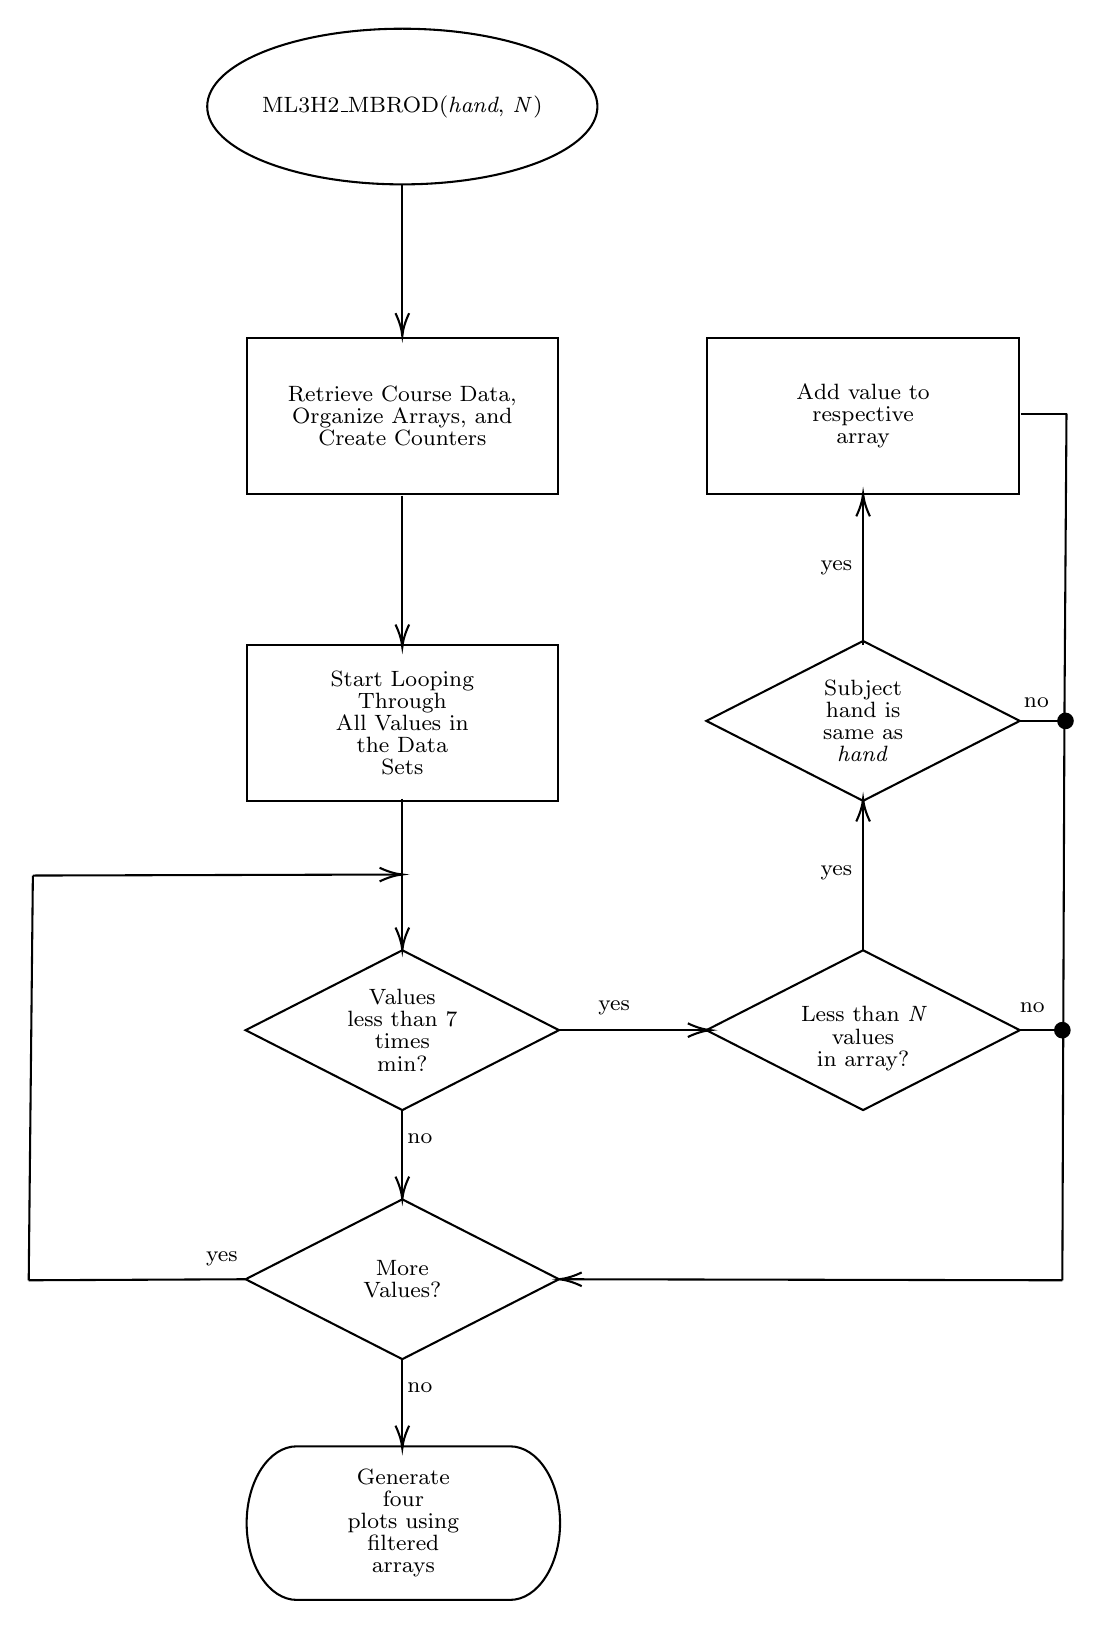
\begin{tikzpicture}[x=0.75pt,y=0.75pt,yscale=-1,xscale=1]
%uncomment if require: \path (0,801); %set diagram left start at 0, and has height of 801

%Shape: Ellipse [id:dp06026735517165571] 
\draw   (229,39.5) .. controls (229,18.79) and (271.09,2) .. (323,2) .. controls (374.91,2) and (417,18.79) .. (417,39.5) .. controls (417,60.21) and (374.91,77) .. (323,77) .. controls (271.09,77) and (229,60.21) .. (229,39.5) -- cycle ;
%Shape: Rectangle [id:dp880516595801381] 
\draw   (248,151) -- (398,151) -- (398,226) -- (248,226) -- cycle ;
%Straight Lines [id:da08375757950130125] 
\draw    (323,77) -- (323,148) ;
\draw [shift={(323,150)}, rotate = 270] [color={rgb, 255:red, 0; green, 0; blue, 0 }  ][line width=0.75]    (10.93,-3.29) .. controls (6.95,-1.4) and (3.31,-0.3) .. (0,0) .. controls (3.31,0.3) and (6.95,1.4) .. (10.93,3.29)   ;
%Flowchart: Decision [id:dp5735470816878454] 
\draw   (323,446) -- (398.5,484.5) -- (323,523) -- (247.5,484.5) -- cycle ;
%Straight Lines [id:da5891435380987948] 
\draw    (323,227) -- (323,298) ;
\draw [shift={(323,300)}, rotate = 270] [color={rgb, 255:red, 0; green, 0; blue, 0 }  ][line width=0.75]    (10.93,-3.29) .. controls (6.95,-1.4) and (3.31,-0.3) .. (0,0) .. controls (3.31,0.3) and (6.95,1.4) .. (10.93,3.29)   ;
%Shape: Rectangle [id:dp1739230692817313] 
\draw   (248,299) -- (398,299) -- (398,374) -- (248,374) -- cycle ;
%Straight Lines [id:da5912825997995481] 
\draw    (323,373) -- (323,444) ;
\draw [shift={(323,446)}, rotate = 270] [color={rgb, 255:red, 0; green, 0; blue, 0 }  ][line width=0.75]    (10.93,-3.29) .. controls (6.95,-1.4) and (3.31,-0.3) .. (0,0) .. controls (3.31,0.3) and (6.95,1.4) .. (10.93,3.29)   ;
%Shape: Boxed Line [id:dp9932206661848584] 
\draw    (398.5,484.5) -- (469.5,484.5) ;
\draw [shift={(471.5,484.5)}, rotate = 180] [color={rgb, 255:red, 0; green, 0; blue, 0 }  ][line width=0.75]    (10.93,-3.29) .. controls (6.95,-1.4) and (3.31,-0.3) .. (0,0) .. controls (3.31,0.3) and (6.95,1.4) .. (10.93,3.29)   ;
%Flowchart: Decision [id:dp4743967302886527] 
\draw   (545,446) -- (620.5,484.5) -- (545,523) -- (469.5,484.5) -- cycle ;
%Shape: Boxed Line [id:dp2787171518355003] 
\draw    (545,446) -- (545,375) ;
\draw [shift={(545,373)}, rotate = 90] [color={rgb, 255:red, 0; green, 0; blue, 0 }  ][line width=0.75]    (10.93,-3.29) .. controls (6.95,-1.4) and (3.31,-0.3) .. (0,0) .. controls (3.31,0.3) and (6.95,1.4) .. (10.93,3.29)   ;
%Shape: Rectangle [id:dp9152323990484745] 
\draw   (470,151) -- (620,151) -- (620,226) -- (470,226) -- cycle ;
%Flowchart: Decision [id:dp7823778282166178] 
\draw   (323,566) -- (398.5,604.5) -- (323,643) -- (247.5,604.5) -- cycle ;
%Straight Lines [id:da1962915410506696] 
\draw    (641,605) -- (400.5,604.5) ;
\draw [shift={(398.5,604.5)}, rotate = 0.12] [color={rgb, 255:red, 0; green, 0; blue, 0 }  ][line width=0.75]    (10.93,-3.29) .. controls (6.95,-1.4) and (3.31,-0.3) .. (0,0) .. controls (3.31,0.3) and (6.95,1.4) .. (10.93,3.29)   ;
%Straight Lines [id:da8225648760923123] 
\draw    (323,523) -- (323,564) ;
\draw [shift={(323,566)}, rotate = 270] [color={rgb, 255:red, 0; green, 0; blue, 0 }  ][line width=0.75]    (10.93,-3.29) .. controls (6.95,-1.4) and (3.31,-0.3) .. (0,0) .. controls (3.31,0.3) and (6.95,1.4) .. (10.93,3.29)   ;
%Straight Lines [id:da8422962655605244] 
\draw    (620.5,335.5) -- (642.5,335.5) ;
%Straight Lines [id:da04998585252964416] 
\draw    (642,334) -- (641,605) ;
%Straight Lines [id:da43416796211710285] 
\draw    (143,605) -- (247.5,604.5) ;
%Straight Lines [id:da8807304940200649] 
\draw    (145,410) -- (143,605) ;
%Straight Lines [id:da7168272354961771] 
\draw    (145,410) -- (321,409.51) ;
\draw [shift={(323,409.5)}, rotate = 179.84] [color={rgb, 255:red, 0; green, 0; blue, 0 }  ][line width=0.75]    (10.93,-3.29) .. controls (6.95,-1.4) and (3.31,-0.3) .. (0,0) .. controls (3.31,0.3) and (6.95,1.4) .. (10.93,3.29)   ;
%Straight Lines [id:da086039166652641] 
\draw    (620.5,484.5) -- (642.5,484.5) ;
%Shape: Circle [id:dp8414382717513849] 
\draw  [fill={rgb, 255:red, 0; green, 0; blue, 0 }  ,fill opacity=1 ] (637.5,484.5) .. controls (637.5,482.57) and (639.07,481) .. (641,481) .. controls (642.93,481) and (644.5,482.57) .. (644.5,484.5) .. controls (644.5,486.43) and (642.93,488) .. (641,488) .. controls (639.07,488) and (637.5,486.43) .. (637.5,484.5) -- cycle ;
%Straight Lines [id:da878855301686359] 
\draw    (323,643) -- (323,684) ;
\draw [shift={(323,686)}, rotate = 270] [color={rgb, 255:red, 0; green, 0; blue, 0 }  ][line width=0.75]    (10.93,-3.29) .. controls (6.95,-1.4) and (3.31,-0.3) .. (0,0) .. controls (3.31,0.3) and (6.95,1.4) .. (10.93,3.29)   ;
%Flowchart: Terminator [id:dp2386338233145222] 
\draw   (272.16,685) -- (374.84,685) .. controls (388.18,685) and (399,701.57) .. (399,722) .. controls (399,742.43) and (388.18,759) .. (374.84,759) -- (272.16,759) .. controls (258.82,759) and (248,742.43) .. (248,722) .. controls (248,701.57) and (258.82,685) .. (272.16,685) -- cycle ;
%Flowchart: Decision [id:dp008358458821891013] 
\draw   (545,297) -- (620.5,335.5) -- (545,374) -- (469.5,335.5) -- cycle ;
%Straight Lines [id:da32593178252161925] 
\draw    (643,187.5) -- (642,334) ;
%Straight Lines [id:da6520057997434436] 
\draw    (621,187.5) -- (643,187.5) ;
%Shape: Boxed Line [id:dp33684862453830156] 
\draw    (545,299) -- (545,228) ;
\draw [shift={(545,226)}, rotate = 90] [color={rgb, 255:red, 0; green, 0; blue, 0 }  ][line width=0.75]    (10.93,-3.29) .. controls (6.95,-1.4) and (3.31,-0.3) .. (0,0) .. controls (3.31,0.3) and (6.95,1.4) .. (10.93,3.29)   ;
%Shape: Circle [id:dp9060227765996967] 
\draw  [fill={rgb, 255:red, 0; green, 0; blue, 0 }  ,fill opacity=1 ] (639,335.5) .. controls (639,333.57) and (640.57,332) .. (642.5,332) .. controls (644.43,332) and (646,333.57) .. (646,335.5) .. controls (646,337.43) and (644.43,339) .. (642.5,339) .. controls (640.57,339) and (639,337.43) .. (639,335.5) -- cycle ;

% Text Node
\draw (323,39.5) node  [font=\tiny] [align=left] {{\footnotesize ML3H2\_MBROD(\textit{hand}, \textit{N})}};
% Text Node
\draw (323,188.5) node  [font=\scriptsize] [align=left] {\begin{minipage}[lt]{99.59pt}\setlength\topsep{0pt}
\begin{center}
{\footnotesize Retrieve Course Data, }\\{\footnotesize Organize Arrays, and Create Counters}
\end{center}

\end{minipage}};
% Text Node
\draw (323,604.5) node  [font=\scriptsize] [align=left] {\begin{minipage}[lt]{37.44pt}\setlength\topsep{0pt}
\begin{center}
{\footnotesize More Values?}
\end{center}

\end{minipage}};
% Text Node
\draw (323,336.5) node  [font=\scriptsize] [align=left] {\begin{minipage}[lt]{59.3pt}\setlength\topsep{0pt}
\begin{center}
{\footnotesize Start Looping Through}\\{\footnotesize All Values in the Data}\\{\footnotesize Sets}
\end{center}

\end{minipage}};
% Text Node
\draw (323,484.5) node  [font=\scriptsize] [align=left] {\begin{minipage}[lt]{45.45pt}\setlength\topsep{0pt}
\begin{center}
{\footnotesize Values}\\{\footnotesize less than 7 times}\\{\footnotesize min?}
\end{center}

\end{minipage}};
% Text Node
\draw (545,188.5) node  [font=\scriptsize] [align=left] {\begin{minipage}[lt]{61.92pt}\setlength\topsep{0pt}
\begin{center}
{\footnotesize Add value to respective}\\{\footnotesize array}
\end{center}

\end{minipage}};
% Text Node
\draw (545,488.5) node  [font=\scriptsize] [align=left] {\begin{minipage}[lt]{51.18pt}\setlength\topsep{0pt}
\begin{center}
{\footnotesize Less than \textit{N} values}\\{\footnotesize in array?}
\end{center}

\end{minipage}};
% Text Node
\draw (324,533) node [anchor=north west][inner sep=0.75pt]  [font=\footnotesize] [align=left] {no};
% Text Node
\draw (416,469) node [anchor=north west][inner sep=0.75pt]  [font=\footnotesize] [align=left] {yes};
% Text Node
\draw (523,404) node [anchor=north west][inner sep=0.75pt]  [font=\footnotesize] [align=left] {yes};
% Text Node
\draw (227,590) node [anchor=north west][inner sep=0.75pt]  [font=\footnotesize] [align=left] {yes};
% Text Node
\draw (619,470) node [anchor=north west][inner sep=0.75pt]  [font=\footnotesize] [align=left] {no};
% Text Node
\draw (324,653) node [anchor=north west][inner sep=0.75pt]  [font=\footnotesize] [align=left] {no};
% Text Node
\draw (323.5,722) node  [font=\scriptsize] [align=left] {\begin{minipage}[lt]{48.63pt}\setlength\topsep{0pt}
\begin{center}
{\footnotesize Generate four}\\{\footnotesize plots using filtered}\\{\footnotesize arrays}
\end{center}

\end{minipage}};
% Text Node
\draw (545,335.5) node  [font=\scriptsize] [align=left] {\begin{minipage}[lt]{41.67pt}\setlength\topsep{0pt}
\begin{center}
{\footnotesize Subject hand is}\\{\footnotesize same as \textit{hand}}
\end{center}

\end{minipage}};
% Text Node
\draw (523,257) node [anchor=north west][inner sep=0.75pt]  [font=\footnotesize] [align=left] {yes};
% Text Node
\draw (621,323) node [anchor=north west][inner sep=0.75pt]  [font=\footnotesize] [align=left] {no};


\end{tikzpicture}
